\documentclass{vilniustech-en}
\vilniustechsetup{
    university={Vilnius Gediminas technical university},
    faculty={Faculty of Fundamental Sciences},
    cathedral={Department of Information Systems},
    workTitle={Malware Analysis Methods},
    workType={Laboratory Work 1},
    workAuthorName={Aurimas Šakalys},
    workAuthorGroup={ITSfm-22},
    workRecipient={lecturer Vitalijus Gurčinas}
}
\addbibresource{bibliography.bib}
\VTDocumentBegin


\section{Initial Setup}

\subsection{Laboratory Environment Setup}

\subsubsection{Malware uploading procedure}

Currently, the way that malware is introduced into the virtual machines are though \textit{Virtual Box} shared folders (\autoref{fig:windows_shared_hyper}, \autoref{fig:linux_shared_hyper}), that are mounted within the virtual machines (\autoref{fig:windows_shared_vm}, \autoref{fig:linux_shared_vm}). The mounts are read-only from the perspective of the virtual machine, which reduces the attack surface for the malware.

\begin{figure}[H]
\begin{center}
    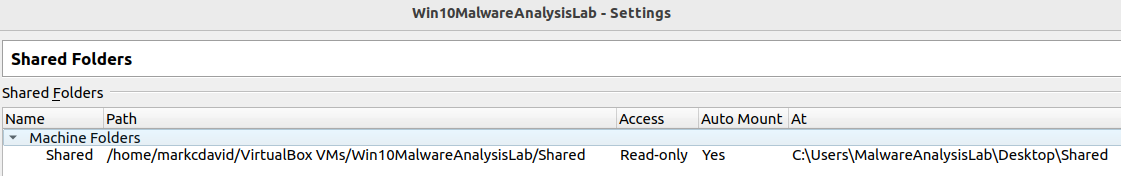
\includegraphics[width=16cm]{img/windows_shared_hyper.png}
    \caption{\textit{FLARE VM} shared folder configuration within \textit{Virtual Box}}
    \label{fig:windows_shared_hyper}
\end{center}
\end{figure}

\begin{figure}[H]
\begin{center}
    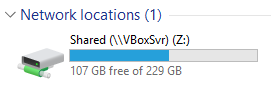
\includegraphics[width=10cm]{img/windows_shared_vm.png}
    \caption{Shared folder within \textit{FLARE VM}}
    \label{fig:windows_shared_vm}
\end{center}
\end{figure}

\begin{figure}[H]
\begin{center}
    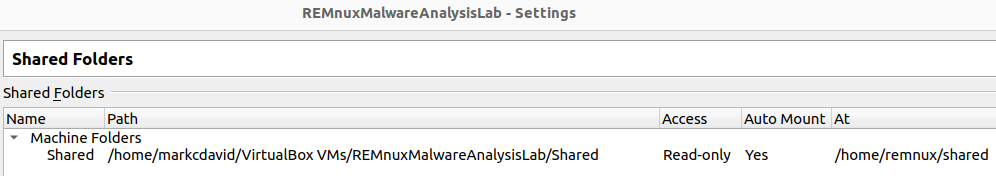
\includegraphics[width=16cm]{img/linux_shared_hyper.png}
    \caption{\textit{REMnux} shared folder configuration within \textit{Virtual Box}}
    \label{fig:linux_shared_hyper}
\end{center}
\end{figure}

\begin{figure}[H]
\begin{center}
    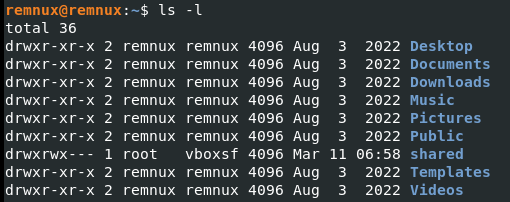
\includegraphics[width=16cm]{img/linux_shared_vm.png}
    \caption{Shared folder within \textit{REMnux}}
    \label{fig:linux_shared_vm}
\end{center}
\end{figure}

\subsubsection{Future Considerations}
While this task is mostly static analysis, where large log files and etc. are not generated, in the future we might need to extradite data from within the virtual machines, without providing them with access to the internet.

Consideration is as follows - provide a host-only network, where the guest can only communicate with the host and configure the host firewall to only allow traffic that the host initiated over \textit{ssh} for \textit{scp} protocol to work.

I have yet to figure out how to configure this, but I think for future tasks this will be useful.

\subsection{Picking the set of malware}

We will be picking the malware from \textit{theZoo} (\autoref{fig:theZoo}). \textit{theZoo} is a project where multiple malware samples are collected for the purposes of malware analysis. They are all stored encryped, have related metadata that allows you to select specific type of malware that you might require.

\begin{figure}[H]
\begin{center}
    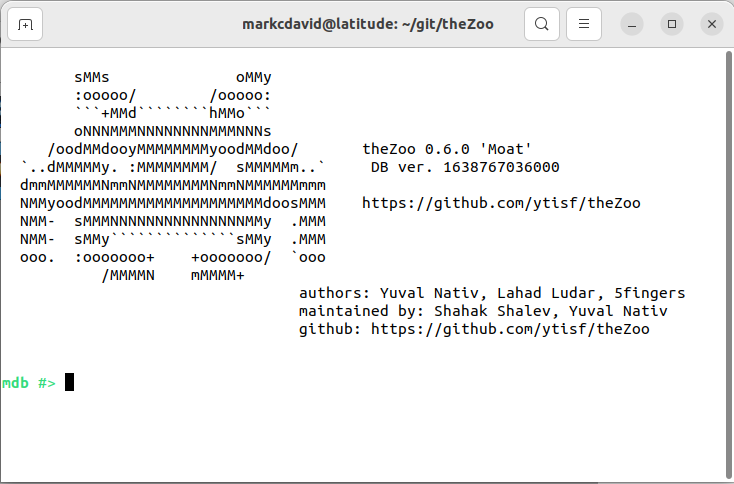
\includegraphics[width=16cm]{img/theZoo.png}
    \caption{TUI for \textit{theZoo}}
    \label{fig:theZoo}
\end{center}
\end{figure}

We will pick one malware for \textit{Linux}, as it seems that \textit{theZoo} could only find one malware sample for \textit{Linux} (\autoref{fig:theZoo_linux}). Manual checking shows that there are more samples for \textit{Linux} systems within \textit{theZoo}, the search simply does not show them. 

\textit{theZoo} search provides us with more malware samples for \textit{Win32} platform (\autoref{fig:theZoo_windows}).

\begin{figure}[H]
\begin{center}
    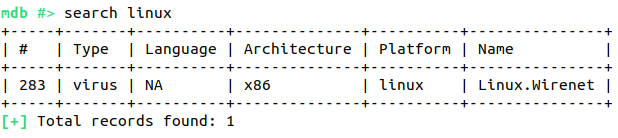
\includegraphics[width=16cm]{img/theZoo_linux.png}
    \caption{theZoo search results for Linux}
    \label{fig:theZoo_linux}
\end{center}
\end{figure}


\begin{figure}[H]
\begin{center}
    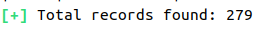
\includegraphics[width=8cm]{img/theZoo_windows.png}
    \caption{\textit{theZoo} search results for \textit{Win32}}
    \label{fig:theZoo_windows}
\end{center}
\end{figure}

We will choose 3 samples from this set - one worm (\autoref{fig:theZoo_worm}), one trojan (\autoref{fig:theZoo_RAT}), and one ransomware (\autoref{fig:theZoo_ransom}).

\begin{figure}[H]
\begin{center}
    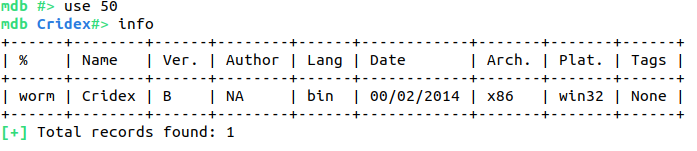
\includegraphics[width=16cm]{img/theZoo_worm.png}
    \caption{\textit{theZoo} information on worm malware}
    \label{fig:theZoo_worm}
\end{center}
\end{figure}

\begin{figure}[H]
\begin{center}
    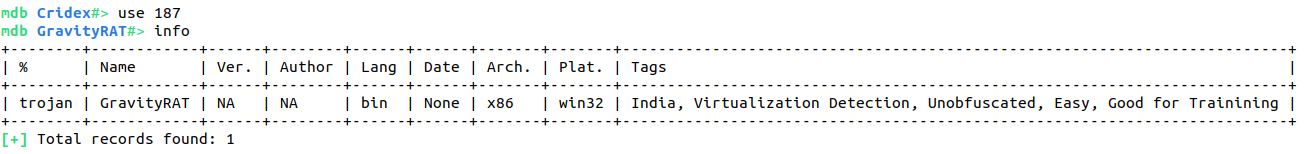
\includegraphics[width=16cm]{img/theZoo_RAT.png}
    \caption{\textit{theZoo} information on trojan malware}
    \label{fig:theZoo_RAT}
\end{center}
\end{figure}

\begin{figure}[H]
\begin{center}
    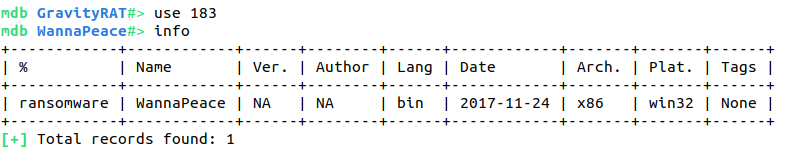
\includegraphics[width=16cm]{img/theZoo_ransom.png}
    \caption{\textit{theZoo} information on ransomware malware}
    \label{fig:theZoo_ransom}
\end{center}
\end{figure}

All the samples are moved to the virtual machines via the shared folders (\autoref{fig:theZoo_within_linux}, \autoref{fig:theZoo_within_windows}).

\begin{figure}[H]
\begin{center}
    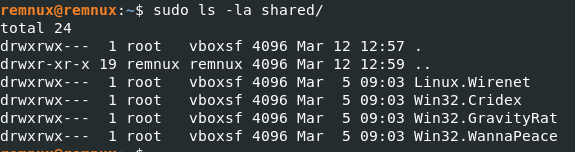
\includegraphics[width=16cm]{img/theZoo_within_linux.png}
    \caption{Malware within \textit{REMnux}}
    \label{fig:theZoo_within_linux}
\end{center}
\end{figure}

\begin{figure}[H]
\begin{center}
    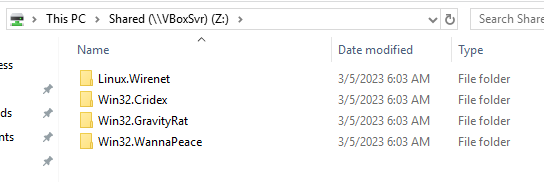
\includegraphics[width=16cm]{img/theZoo_within_windows.png}
    \caption{Malware within \textit{FLARE VM}}
    \label{fig:theZoo_within_windows}
\end{center}
\end{figure}

\section{Task 1}

For malware scanning in \textit{FLARE VM} we will use a free version of \textit{Malwarebytes} software (\autoref{fig:malware_bytes}).

\begin{figure}[H]
\begin{center}
    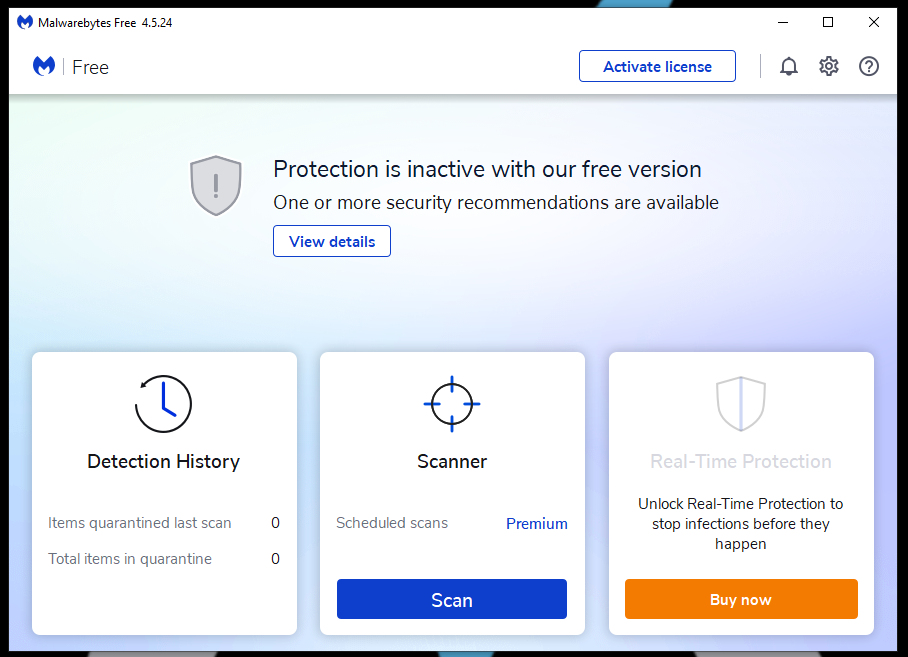
\includegraphics[width=16cm]{img/malware_bytes.png}
    \caption{\textit{Malwarebytes} software}
    \label{fig:malware_bytes}
\end{center}
\end{figure}

Within \textit{REMnux}, we shall use \textit{ClamAV} software. For the default installation of \textit{REMnux}, \textit{ClamAV} does not have any malware database present, as such, we need to fetch the databases using the \textit{freshclam} command (\autoref{fig:clamav}).

\begin{figure}[H]
\begin{center}
    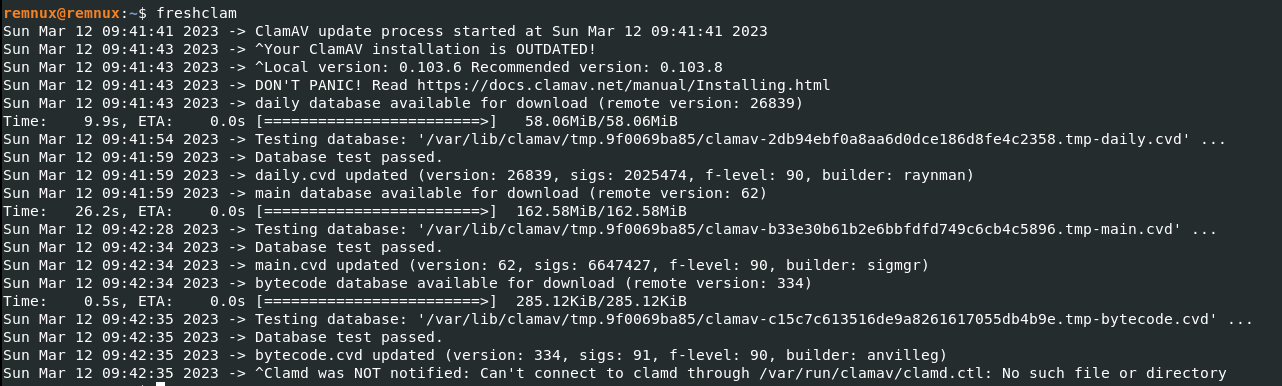
\includegraphics[width=16cm]{img/clamav.png}
    \caption{\textit{ClamAV} database update}
    \label{fig:clamav}
\end{center}
\end{figure}

Although we could run \textit{clamd} daemon, so that the \textit{clamscan} would run a little faster, as we will not be performing a multitude of scans within the system, the performance loss (\autoref{fig:clamav_time}) is not as significant.
\begin{figure}[H]
\begin{center}
    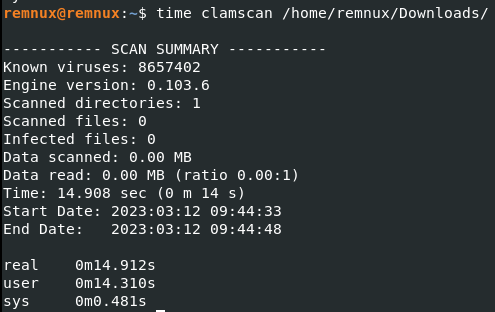
\includegraphics[width=16cm]{img/clamav_time.png}
    \caption{\textit{ClamAV} database loading and scan time}
    \label{fig:clamav_time}
\end{center}
\end{figure}

\section{Task 2}

\textit{Malwarebytes} has identified $\frac{3}{4}$ malware samples (\autoref{fig:malwarebytes_scan_app}). All \textit{Win32} malware samples were identified correctly, while \textit{Linux} malware was not identfied as malware (\autoref{fig:malwarebytes_scan_report}).

\begin{figure}[H]
\begin{center}
    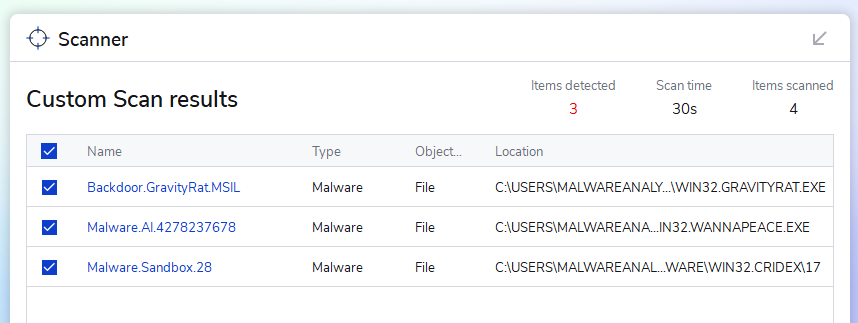
\includegraphics[width=16cm]{img/malwarebytes_scan_app.png}
    \caption{\textit{Malwarebytes} scan within the application}
    \label{fig:malwarebytes_scan_app}
\end{center}
\end{figure}

\begin{figure}[H]
\begin{center}
    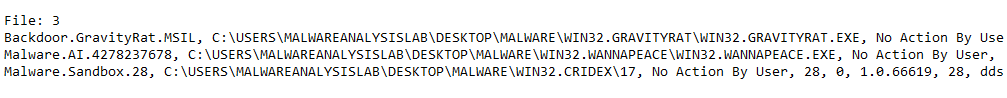
\includegraphics[width=16cm]{img/malwarebytes_scan_report.png}
    \caption{\textit{Malwarebytes} scan report}
    \label{fig:malwarebytes_scan_report}
\end{center}
\end{figure}

\textit{clamscan}, like \textit{Malwarebytes}, managed to indentify $\frac{3}{4}$ malware samples (\autoref{fig:clamav_scan}), but it identified different samples.

It did manage to identify the malware for \textit{Linux} system. It did miss the \textit{Win32.WannaPeace} ransomware malware.

\begin{figure}[H]
\begin{center}
    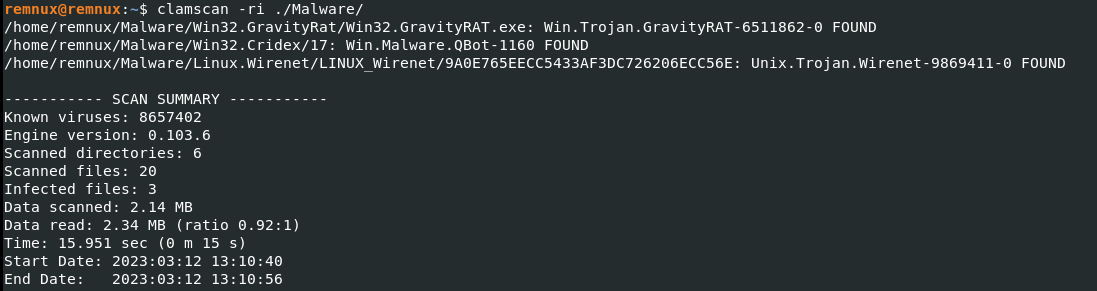
\includegraphics[width=16cm]{img/clamav_scan.png}
    \caption{\textit{ClamAV} scan report}
    \label{fig:clamav_scan}
\end{center}
\end{figure}

\section{Task 3 \& Task 4}

We have submited all four malware samples to \textit{VirusTotal} and got the results.

\textit{Linux.Wirenet} is identified as a virus by \textit{theZoo} (\autoref{fig:theZoo_linux}), while \textit{VirusTotal} identifies it as a trojan (\autoref{fig:virustotal_wirenet}).

\begin{figure}[H]
\begin{center}
    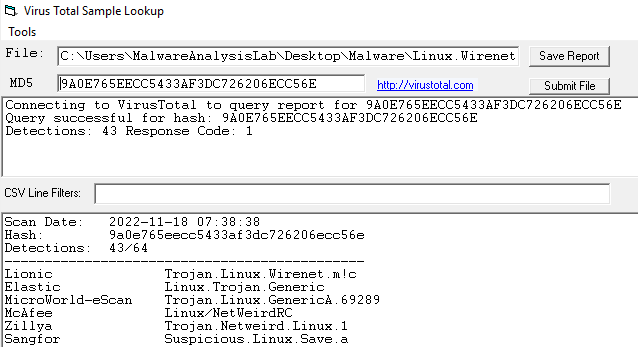
\includegraphics[width=16cm]{img/virustotal_wirenet.png}
    \caption{\textit{VirusTotal} report for \textit{Linux.Wirenet}}
    \label{fig:virustotal_wirenet}
\end{center}
\end{figure}

\textit{Win32.Cridex} is identified as a virus by \textit{theZoo} (\autoref{fig:theZoo_worm}), while \textit{VirusTotal} identifies it as a trojan (\autoref{fig:virustotal_cridex}).

\begin{figure}[H]
\begin{center}
    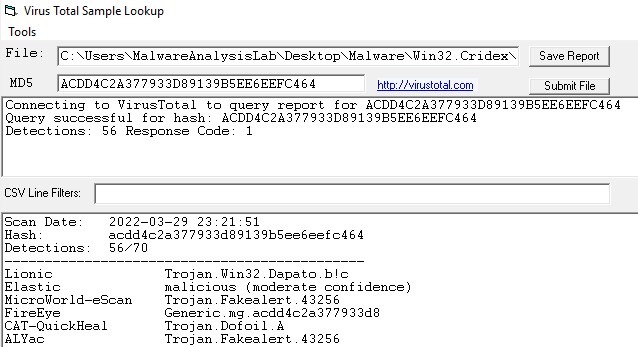
\includegraphics[width=16cm]{img/virustotal_cridex.png}
    \caption{\textit{VirusTotal} report for \textit{Win32.Cridex}}
    \label{fig:virustotal_cridex}
\end{center}
\end{figure}

\textit{Win32.GravityRAT} is identified as a worm by \textit{theZoo} (\autoref{fig:theZoo_RAT}), while \textit{VirusTotal} identifies it as a trojan (\autoref{fig:virustotal_gravityrat}).

\begin{figure}[H]
\begin{center}
    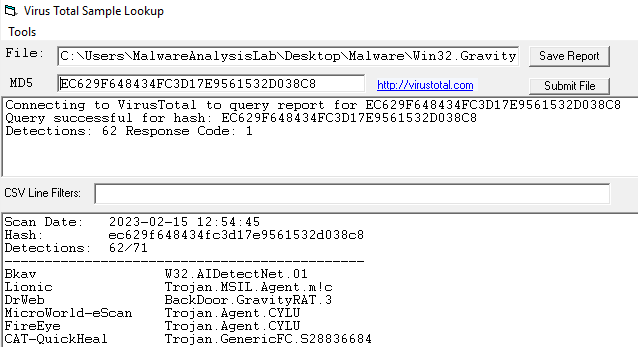
\includegraphics[width=16cm]{img/virustotal_gravityrat.png}
    \caption{\textit{VirusTotal} report for \textit{Win32.GravityRAT}}
    \label{fig:virustotal_gravityrat}
\end{center}
\end{figure}

\textit{Win32.WannaPeace} is identified as a ransomware by \textit{theZoo} (\autoref{fig:theZoo_ransom}), while \textit{VirusTotal} identifies it as a trojan or ransomware (\autoref{fig:virustotal_wannapeace}).

\begin{figure}[H]
\begin{center}
    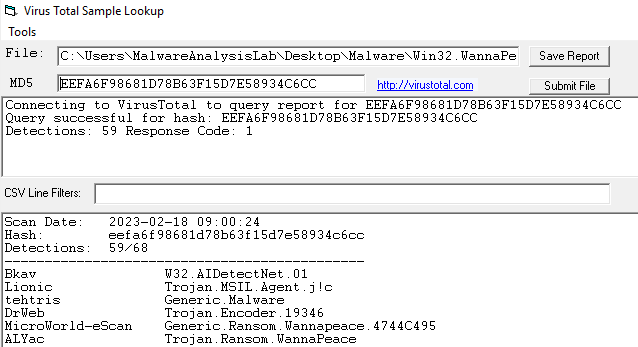
\includegraphics[width=16cm]{img/virustotal_wannapeace.png}
    \caption{\textit{VirusTotal} report for \textit{Win32.WannaPeace}}
    \label{fig:virustotal_wannapeace}
\end{center}
\end{figure}


\section{Task 5 \& Task 6} \label{sec:task5_6}

Tasks 5 and 6 are combined, as we will use multiple tools in our disposal to determine possible behaviour and characteristics of the malware, that includes PE header information gathering. 

We will analyse \textit{Win32.Cridex} and \textit{Win32.WannaPeace} malware.

\subsection{\textit{Win32.Cridex}}

First step that we will take, is to check whether the malware is packed or not. We will use \textit{peid} for this.

\begin{figure}[H]
\begin{center}
    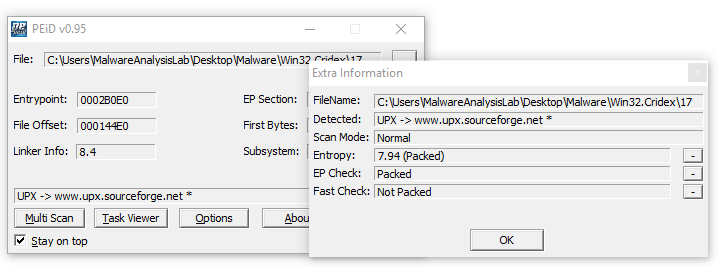
\includegraphics[width=16cm]{img/cridex_peid.png}
    \caption{\textit{peid} report on \textit{Win32.Cridex}}
    \label{fig:cridex_peid}
\end{center}
\end{figure}

The software provides us with the information that it has a high entropy (\autoref{fig:cridex_peid}), which is indicative of a packed malware. Additionally, it has detected, that UPX has been used to pack the software. As such, it's likely that we will be able to unpack the software.

The reason we want to unpack the software, is that we will not be able to use static analysis tools to investigate what type of behaviour the malware might have if it is packed.

\begin{figure}[H]
\begin{center}
    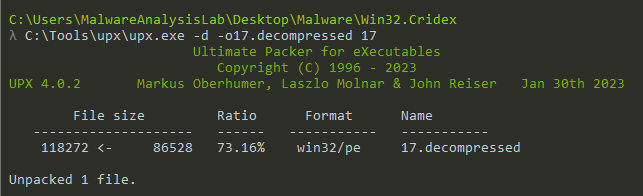
\includegraphics[width=16cm]{img/cridex_unpack.png}
    \caption{Unpacking \textit{Win32.Cridex} with \textit{UPX}}
    \label{fig:cridex_unpack}
\end{center}
\end{figure}

We have used UPX to unpack the malware and it worked successfully (\autoref{fig:cridex_unpack}).

\begin{figure}[H]
\begin{center}
    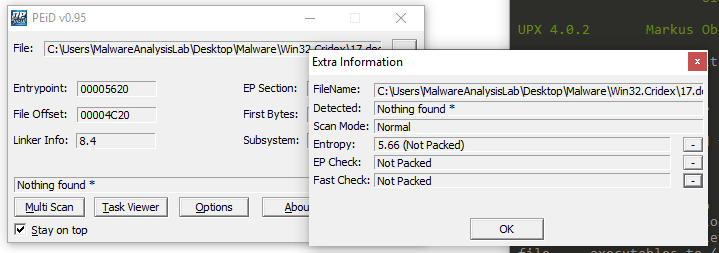
\includegraphics[width=16cm]{img/cridex_peid_unpack.png}
    \caption{\textit{peid} report on \textit{Win32.Cridex} after unpacking}
    \label{fig:cridex_peid_unpack}
\end{center}
\end{figure}

Getting information using \textit{peid} we can see that the entropy had gotten down (\autoref{fig:cridex_peid_unpack}), which is indicative of software not being packed. Additionally, \textit{peid} does not detect any packer. As such, we have malware that has been unpacked and we will be capable of performing analysis on it's behaviour.

Using \textit{strings} we do not get much information, it seems that the malware contains a lot of randomly generated unicode strings (\autoref{fig:cridex_strings}).

\begin{figure}[H]
\begin{center}
    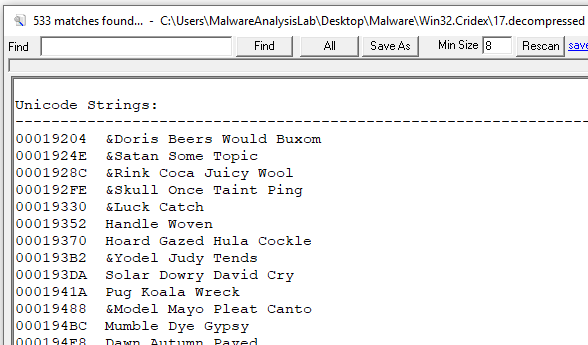
\includegraphics[width=16cm]{img/cridex_strings.png}
    \caption{strings report on unpacked Win32.Cridex}
    \label{fig:cridex_strings}
\end{center}
\end{figure}

Using \textit{CFF Explorer} we can see that the malware only uses a few libraries (\autoref{fig:cridex_cff}).
\begin{figure}[H]
\begin{center}
    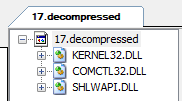
\includegraphics[width=10cm]{img/cridex_cff.png}
    \caption{\textit{CFF Explorer} dependency report on unpacked \textit{Win32.Cridex}}
    \label{fig:cridex_cff}
\end{center}
\end{figure}

To make our work a bit easier, we will use \textit{Ghidra} to analyse the malware and provide us with the function calls to these libraries. Using these we could determine a few characteristics about the malware.

\textit{Ghidra}, after analysing the malware, shows us that the malware uses \textit{LoadLibraryW} and \textit{LoadLibraryExW} API calls (\autoref{fig:cridex_ghidra}).

\begin{figure}[H]
\begin{center}
    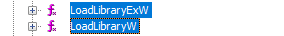
\includegraphics[width=10cm]{img/cridex_ghidra.png}
    \caption{\textit{Ghida} report on used API calls in unpacked \textit{Win32.Cridex}}
    \label{fig:cridex_ghidra}
\end{center}
\end{figure}

This means that the malware could possibly dynamically load libraries and this does not provide an indication as to what the behaviour of the malware is. The next steps would be to either do full reverse engineering or perform dynamic analysis and run the sample. We shall skip these steps for now.

\subsection{\textit{Win32.WannaPeace}}

We shall run a similar procedure for the \textit{Win32.WannaPeace} malware.

Using \textit{peid} we can find an indication, that the malware is packed (\autoref{fig:wannapeace_peid}). 

\begin{figure}[H]
\begin{center}
    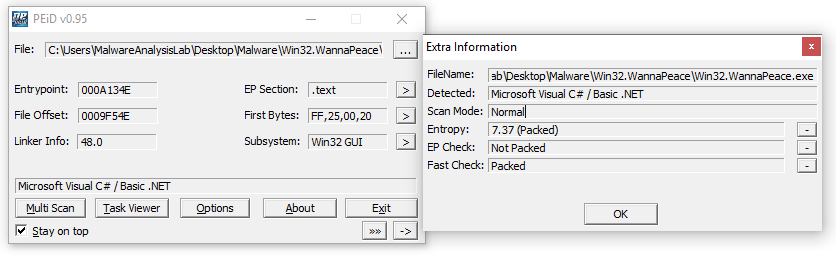
\includegraphics[width=16cm]{img/wannapeace_peid.png}
    \caption{\textit{peid} report on \textit{Win32.WannaPeace}}
    \label{fig:wannapeace_peid}
\end{center}
\end{figure}

Additionally, we can see an indication that this is a \textit{.NET} executable (\autoref{fig:wannapeace_peid}), which should allow us to try to analyse the malware using \textit{dnSpy}. 

\begin{figure}[H]
\begin{center}
    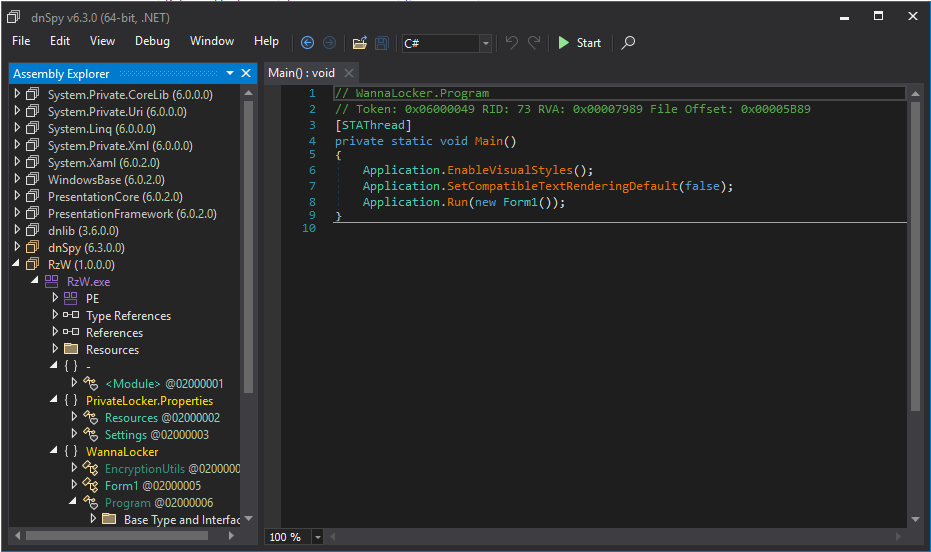
\includegraphics[width=16cm]{img/wannapeace_dnspy_main.png}
    \caption{Main function of \textit{Win32.WannaPeace}}
    \label{fig:wannapeace_dnspy_main}
\end{center}
\end{figure}

We can see that the malware is a \textit{WinForms} application. The \textit{Main} method (\autoref{fig:wannapeace_dnspy_main}) simply creates the new form and that would seem to be the entire functionality (\autoref{fig:wannapeace_dnspy_form_init}).

\begin{figure}[H]
\begin{center}
    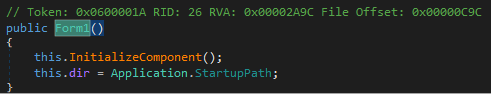
\includegraphics[width=16cm]{img/wannapeace_dnspy_form_init.png}
    \caption{Main form initialisation of \textit{Win32.WannaPeace}}
    \label{fig:wannapeace_dnspy_form_init}
\end{center}
\end{figure}

We are partially cheating here, as we do know this is a ransomware type of malware, as such, we would expect the users filesystem to be encrypted prior to the execution of the form that asks for the ransom. Where would we be able to find it?

We can find a namespace/class for encryption utilities, and it has functions for encrypting files and directories (\autoref{fig:wannapeace_dnspy_crypto}). 

\begin{figure}[H]
\begin{center}
    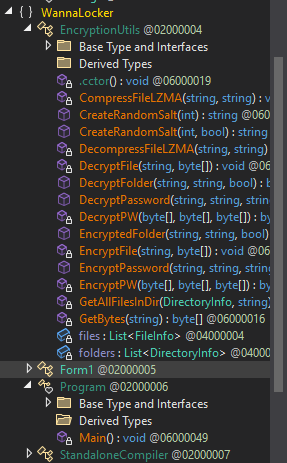
\includegraphics[width=8cm]{img/wannapeace_dnspy_crypto.png}
    \caption{Cryptographic helper functions of \textit{Win32.WannaPeace}}
    \label{fig:wannapeace_dnspy_crypto}
\end{center}
\end{figure}

We want to determine, where the usage of these functions begin. If we look at the usages of \textit{EncryptFolder} function, we can see that it is used from a \textit{bgw\_DoWork} method (\autoref{fig:wannapeace_bgw}). 

\begin{figure}[H]
\begin{center}
    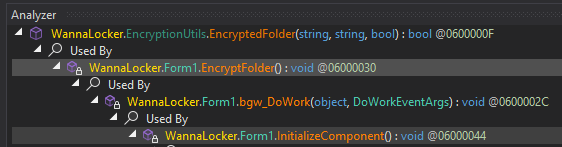
\includegraphics[width=16cm]{img/wannapeace_bgw.png}
    \caption{Usage tree for \textit{EncryptFolder} function in \textit{Win32.WannaPeace}}
    \label{fig:wannapeace_bgw}
\end{center}
\end{figure}

\textit{bgw}, usually stands for background worker, and the \textit{DoWork} postfix provides us some indication that this might be true. 


\begin{figure}[H]
\begin{center}
    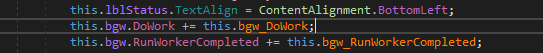
\includegraphics[width=16cm]{img/wannapeace_bgw_subscribe.png}
    \caption{Background worker method subscription in \textit{Win32.WannaPeace}}
    \label{fig:wannapeace_bgw_subscribe}
\end{center}
\end{figure}

\begin{figure}[H]
\begin{center}
    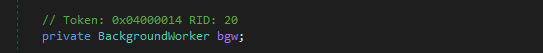
\includegraphics[width=16cm]{img/wannapeace_bgw_store.png}
    \caption{Background worker variable in \textit{Win32.WannaPeace}}
    \label{fig:wannapeace_bgw_store}
\end{center}
\end{figure}

\begin{figure}[H]
\begin{center}
    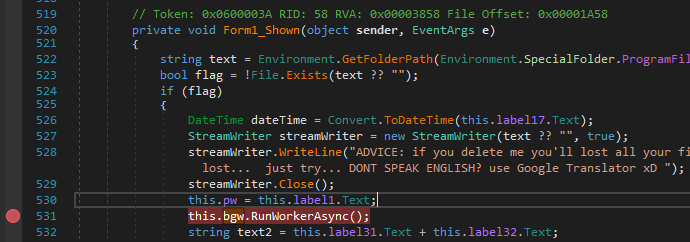
\includegraphics[width=16cm]{img/wannapeace_bgw_usage.png}
    \caption{Usage of the background worker in \textit{Win32.WannaPeace}}
    \label{fig:wannapeace_bgw_usage}
\end{center}
\end{figure}

We can see that the background worker (\autoref{fig:wannapeace_bgw_store}) is created during composition of the form (\autoref{fig:wannapeace_bgw_subscribe}) and when the form is first shown it launches the worker (\autoref{fig:wannapeace_bgw_usage}), which in turn - encrypts the users files.

\textit{bgw2\_DoWork} (\autoref{fig:wannapeace_bgw2}) launches the decryption algorithm, but it only launches if user provides correct password for the decryption (\autoref{fig:wannapeace_bgw2_usage}).

\begin{figure}[H]
\begin{center}
    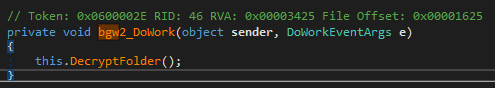
\includegraphics[width=16cm]{img/wannapeace_bgw2.png}
    \caption{Subsciption method for second background worker in \textit{Win32.WannaPeace}}
    \label{fig:wannapeace_bgw2}
\end{center}
\end{figure}

\begin{figure}[H]
\begin{center}
    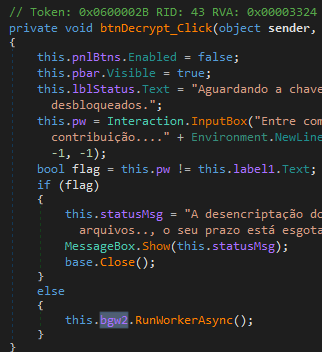
\includegraphics[width=10cm]{img/wannapeace_bgw2_usage.png}
    \caption{Behaviour code for second background worker in \textit{Win32.WannaPeace}}
    \label{fig:wannapeace_bgw2_usage}
\end{center}
\end{figure}

\section{Task 7}

We will use \textit{In Shadow Batch Virus Generator} to generate our malware.

\begin{figure}[H]
\begin{center}
    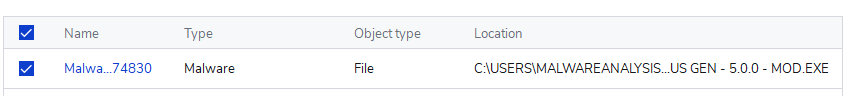
\includegraphics[width=16cm]{img/malware_gen_scan.png}
    \caption\textit{Malwarebytes} scan result for \textit{In Shadow Batch Virus Generator}
    \label{fig:malware_gen_scan}
\end{center}
\end{figure}

The generator itself is being marked as malware (\autoref{fig:malware_gen_scan}). \textit{peid} provides us with information, that this is a \textit{.NET} executable (\autoref{fig:malware_gen_peid}), which means we could check for untoward behaviour with \textit{dnSpy} as well.

\begin{figure}[H]
\begin{center}
    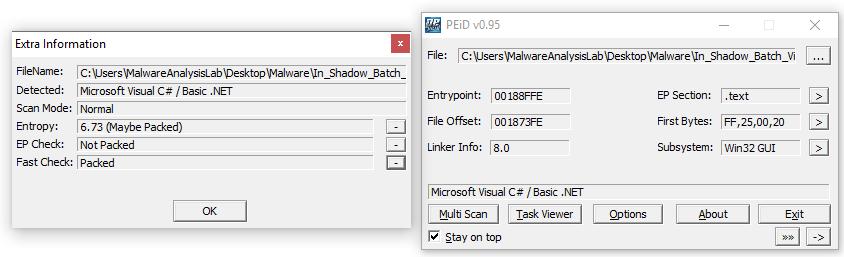
\includegraphics[width=16cm]{img/malware_gen_peid.png}
    \caption{\textit{peid} report on \textit{In Shadow Batch Virus Generator}}
    \label{fig:malware_gen_peid}
\end{center}
\end{figure}

A quick analysis using \textit{dnSpy} shows that the software does not seem to be malicous and at most it simply generates a batch file using snippets within resources (\autoref{fig:malware_gen_resource}) or code itself (\autoref{fig:malware_gen_behaviour}).
As the software is deemed safe to use, we shall proceed.

\begin{figure}[H]
\begin{center}
    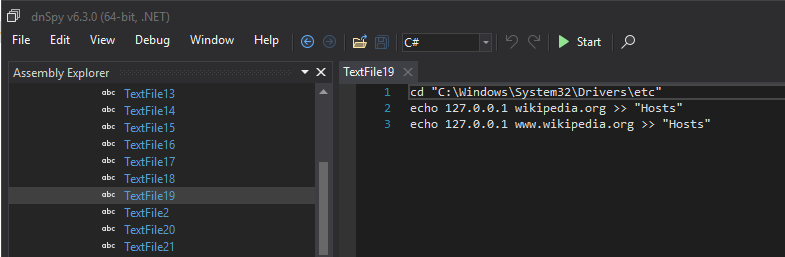
\includegraphics[width=16cm]{img/malware_gen_resource.png}
    \caption{Resources file within \textit{In Shadow Batch Virus Generator}}
    \label{fig:malware_gen_resource}
\end{center}
\end{figure}


\begin{figure}[H]
\begin{center}
    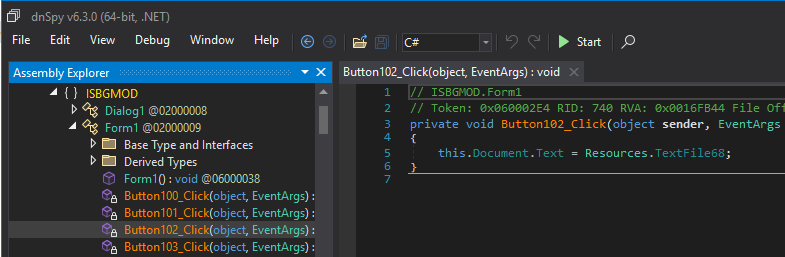
\includegraphics[width=16cm]{img/malware_gen_behaviour.png}
    \caption{Behaviour of a button click function within \textit{In Shadow Batch Virus Generator}}
    \label{fig:malware_gen_behaviour}
\end{center}
\end{figure}


\subsection{Fun Aside}
Apparantly, this software has easter eggs within it (\autoref{fig:malware_gen_easter_egg}). As easter eggs are considered to be malicious, this software could now be classified as malware.

\begin{figure}[H]
\begin{center}
    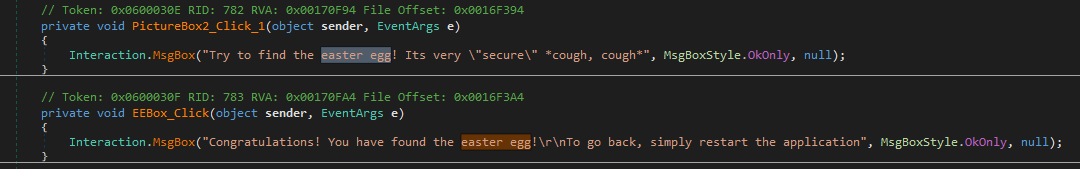
\includegraphics[width=16cm]{img/malware_gen_easter_egg.png}
    \caption{Indication of an easter egg within \textit{In Shadow Batch Virus Generator}}
    \label{fig:malware_gen_easter_egg}
\end{center}
\end{figure}

\subsection{Generated Malware}
Using the generator, a sample malicous batch file has been created (\autoref{fig:generated_malware}). 
\begin{figure}[H]
\begin{center}
    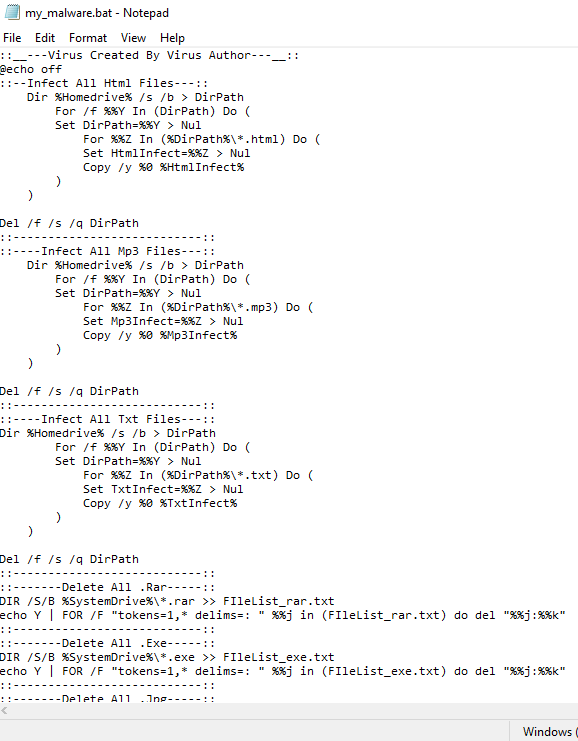
\includegraphics[width=10cm]{img/generated_malware.png}
    \caption{Generated batch file malware}
    \label{fig:generated_malware}
\end{center}
\end{figure}

Additionally, \textit{Malwarebytes} does not detect it as a malicous software (\autoref{fig:malwarebytes_generated_scan}).
\begin{figure}[H]
\begin{center}
    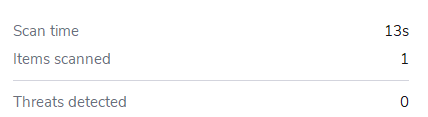
\includegraphics[width=16cm]{img/malwarebytes_generated_scan.png}
    \caption{Scan of the generated batch malware}
    \label{fig:malwarebytes_generated_scan}
\end{center}
\end{figure}

\section{Task 8} \label{sec:task8}

For this task, we shall cheat a little, and use a \textit{Win32.Cridex} malware sample that we unpacked in Task 5/6. We can check, that both the packed and unpacked malware is detected by \textit{Malwarebytes} (\autoref{fig:mawlarebytes_scan_unpacked}).  

\begin{figure}[H]
\begin{center}
    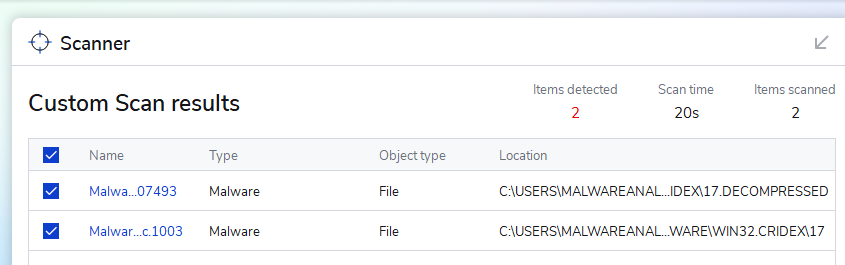
\includegraphics[width=16cm]{img/mawlarebytes_scan_unpacked.png}
    \caption{Scan of \textit{Win32.Cridex} malware}
    \label{fig:mawlarebytes_scan_unpacked}
\end{center}
\end{figure}

We have used \textit{UPX} to pack the file (\autoref{fig:packing_process_max_compression}). We can see that the file now has a similar size (\autoref{fig:packing_similar_size}). Let's check the hashes of the files to ensure that we have not created the exact same files.

\begin{figure}[H]
\begin{center}
    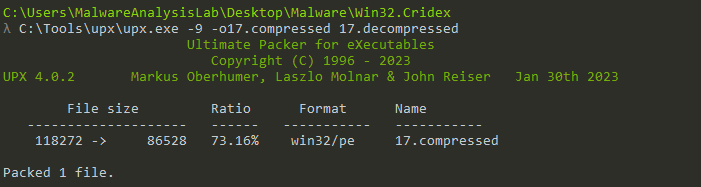
\includegraphics[width=16cm]{img/packing_process_max_compression.png}
    \caption{Packing of the \textit{Win32.Cridex} malware}
    \label{fig:packing_process_max_compression}
\end{center}
\end{figure}

\begin{figure}[H]
\begin{center}
    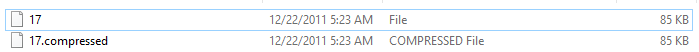
\includegraphics[width=16cm]{img/packing_similar_size.png}
    \caption{Indication of similar sized executables}
    \label{fig:packing_similar_size}
\end{center}
\end{figure}

\textit{HashMyFiles} software provides us with hashes for both malware and we can see that it is indeed different (\autoref{fig:packing_hash}). 

\begin{figure}[H]
\begin{center}
    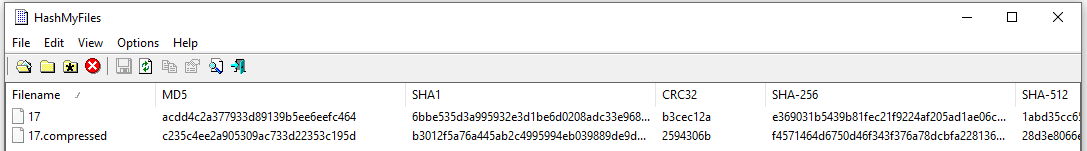
\includegraphics[width=16cm]{img/packing_hash.png}
    \caption{Hash of packed malware}
    \label{fig:packing_hash}
\end{center}
\end{figure}

If it had been the same, we could have used a different level of compression via \textit{UPX} (e.g. -1 instead of -9), to get a less compressed (\autoref{fig:packing_process_min_compression}), but different file (\autoref{fig:packing_size_hash}).

\begin{figure}[H]
\begin{center}
    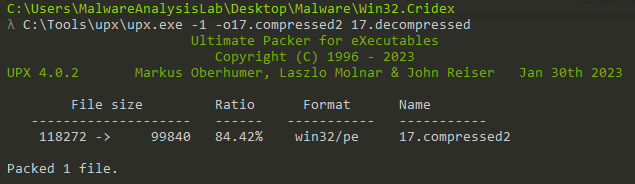
\includegraphics[width=16cm]{img/packing_process_min_compression.png}
    \caption{Packing process with smaller compression rate}
    \label{fig:packing_process_min_compression}
\end{center}
\end{figure}

\begin{figure}[H]
\begin{center}
    \includegraphics[width=16cm]{img/packing_size_hash.png}
    \caption{Hashes of differently packed malware}
    \label{fig:packing_size_hash}
\end{center}
\end{figure}

As we can see, after rescanning the malware samples, the newly packed malware samples are not detected anymore by \textit{Malwarebytes} (\autoref{fig:scan_of_repacked_malware}).

\begin{figure}[H]
\begin{center}
    \includegraphics[width=16cm]{img/scan_of_repacked_malware.png}
    \caption{Scan of packed malware}
    \label{fig:scan_of_repacked_malware}
\end{center}
\end{figure}

\section{Task 9}

For this task, we shall use \textit{Cuckoo Sandbox}, that is hosted online. We can find one like this at \url{cuckoo.cert.ee}. This allows us to forgoe (for now) the need to set up the sandbox ourselves, and will provide us with required data.

We shall analyse \textit{Win32.GravityRAT} (\autoref{fig:cuckoo_rat_scan}) and \textit{Win32.WannaPeace} (\autoref{fig:cuckoo_wannapeace_scan}) malware using \textit{Cuckoo Sandbox}.

\begin{figure}[H]
\begin{center}
    \includegraphics[width=16cm]{img/cuckoo_wannapeace_scan.png}
    \caption{\textit{Cuckoo Sandbox} scan of \textit{Win32.WannaPeace} malware}
    \label{fig:cuckoo_wannapeace_scan}
\end{center}
\end{figure}

\begin{figure}[H]
\begin{center}
    \includegraphics[width=16cm]{img/cuckoo_rat_scan.png}
    \caption{\textit{Cuckoo Sandbox} scan of \textit{Win32.GravityRAT} malware}
    \label{fig:cuckoo_rat_scan}
\end{center}
\end{figure}

We can see the results for both of these malware samples (\autoref{fig:malware_sus}). They scored 10/10, which shows that this malware is extremelly suspicious.

\begin{figure}[H]
\begin{center}
    \includegraphics[width=16cm]{img/malware_sus.png}
    \caption{Suspicion rating for provided malware}
    \label{fig:malware_sus}
\end{center}
\end{figure}

\subsection{\textit{Win32.WannaPeace}}

\textit{Cuckoo} is capable of providing a lot of information that we would collect in one area (PE headers, section sizes, entropy etc.). While these could be useful for analysis, the sandbox provides a summary of actions and behaviours taken by the malware.

\begin{figure}[H]
\begin{center}
    \includegraphics[width=16cm]{img/cuckoo_peace_results.png}
    \caption{Results of \textit{Cuckoo Sandbox} analysis for \textit{Win32.WannaPeace} malware}
    \label{fig:cuckoo_peace_results}
\end{center}
\end{figure}

To begin, this shows an inexperienced malware analyst certain behavioral patterns, that could be useful for future malware analysis efforts (e.g. checking for total memory using \textit{GlobalMemoryStatusEx} to detect virtual machines with low memory). 

As we can see in the results above (\autoref{fig:cuckoo_peace_results}), a lot of indication for suspicion of the file is that it is detected by the malware scanners, not from the behaviour.

It is shown as a packed malware, when in truth it is simply a \textit{.NET CLR} executable, which shows up as packed due to high file entropy.

\textit{Cuckoo} was unable to determine, by behavioral analysis the severity of the malware.

\subsection{\textit{Win32.GravityRAT}}

The results are a bit different with the \textit{Win32.GravityRAT} malware, as it triggers a few more rules within the \textit{Cuckoo Sandbox} (\autoref{fig:cuckoo_rat_results}).

\begin{figure}[H]
\begin{center}
    \includegraphics[width=16cm]{img/cuckoo_rat_results.png}
    \caption{Results of \textit{Cuckoo Sandbox} analysis for \textit{Win32.GravityRAT} malware}
    \label{fig:cuckoo_rat_results}
\end{center}
\end{figure}

The malware exibits a bit more suspicious behaviour, like moving it's own executable to a new location, tries harder to detect if it was ran within a virtual machine and actually sent data back to \textit{CnC} center. 

We can determine that (desipte knowing that the malware is a \textit{RAT}) the malware is capable of obfuscating and hiding itself within the system, sending out data back to \textit{CnC} center, indicating it's a \textit{RAT}.


\section{Additional Work}

For additional work, we need to select three malware obfuscation techniques, test them and provide our insights into their pros and cons.

\subsection{Packing}

Packing has been done previously in the report (Section \ref{sec:task5_6}, Section \ref{sec:task8}). One thing that we have not done with the newly packed malware in those sections was to scan them using VirusTotal. Only providing the hashes to \textit{VirusTotal} we can see that it does not yet contain any information for a file with that hash (\autoref{fig:virustotal_packed_hash_scan}). By uploading the file directly to \textit{VirusTotal}, after static and dynamic analysis is performed, the malware is identified easily (\autoref{fig:virustotal_packed_scan}).

\begin{figure}[H]
\begin{center}
    \includegraphics[width=16cm]{img/virustotal_packed_hash_scan.png}
    \caption{Results of uploading hashes of repacked malware to \textit{VirusTotal}}
    \label{fig:virustotal_packed_hash_scan}
\end{center}
\end{figure}
    
\begin{figure}[H]
\begin{center}
    \includegraphics[width=16cm]{img/virustotal_packed_scan.png}
    \caption{Results of uploading repacked malware to \textit{VirusTotal}}
    \label{fig:virustotal_packed_scan}
\end{center}
\end{figure}

The pros of this method is that it can be realively easy to pack the malware, using some preexisting packers, to manage to skip past the fingerprinting, but it's not as robust against reverse engineering and sandboxing/dynamic analysis of the malware. Even if using some custom packer, the malware analyst could simply run the malware, until it unpacks itself and extract the unpacked malware from memory.

\subsection{Installer}

In this case we shall use \textit{NSIS} installer creation software. We will demonstrate, similarly to packing, that creating an installer would provide us with a method to get past fingerprinting and we will check if automatic dynamic analysis will be able to identify the malware.

For this, we shall use a very simple example script provided, which will allow us to create a very simple installer, but it would work for our purposes (\autoref{fig:installer_default}). This installer simply extracts the malware onto the victims computer. We shall do a test with the calculator app to see if it could launch the application immediately after installation.

\begin{figure}[H]
\begin{center}
    \includegraphics[width=16cm]{img/installer_default.png}
    \caption{Part of the default \textit{NSIS} installer creation script}
    \label{fig:installer_default}
\end{center}
\end{figure}

As expected, after hiding the malware within an installer, we manage to evade fingerprinting detection, but once uploaded to \textit{VirusTotal} for dynamic analysis the malware is immedeately detected (\autoref{fig:installer_scan}). 

\begin{figure}[H]
\begin{center}
    \includegraphics[width=16cm]{img/installer_scan.png}
    \caption{Hash check and dynamic analysis of the malware hidden via an installer}
    \label{fig:installer_scan}
\end{center}
\end{figure}

As a proof of concept, we shall create an installer that would launch the calculator app after installing it (\autoref{fig:calc_launch}). After launching the installer and installing the software we can see that the calculator app launches automatically (\autoref{fig:calc_launch}).

\begin{figure}[H]
\begin{center}
    \includegraphics[width=16cm]{img/install_calc.png}
    \caption{\textit{NSIS} script for installing and launching the calculator app}
    \label{fig:install_calc}
\end{center}
\end{figure}

\begin{figure}[H]
\begin{center}
    \includegraphics[width=16cm]{img/calc_launch.png}
    \caption{Successful launch of the calculator app immediately after installation}
    \label{fig:calc_launch}
\end{center}
\end{figure}

The main pros of this method is that we would be capable of creating an installer for some specific type of software (e.g. a browser), that would install as expected, only to install and launch some malware payload in the background. As mentioned before, we are capable of evading fingerprinting of the malware, not so much the dynamic analysis as the installer performs some curious actions that could be caught by anti-malware software.

\subsection{Encryption}

To test an encryption method, we shall use base64 encoded payload, that a script would extract. Although base64 encoding is not exactly encryption, it would still be pretty close to what the encrypted malware would do - unencrypt (in out case decode) the payload and execute it.

\begin{figure}[H]
\begin{center}
    \includegraphics[width=16cm]{img/malware_base64.png}
    \caption{Encoding of the malware using base64}
    \label{fig:malware_base64}
\end{center}
\end{figure}

\begin{figure}[H]
\begin{center}
    \includegraphics[width=16cm]{img/malware_unpack.png}
    \caption{Unpacking of the malware}
    \label{fig:malware_unpack}
\end{center}
\end{figure}

The proof of concept is done using \textit{python} scripts. The first script simply takes the malware file and encodes its contents in base64 (\autoref{fig:malware_base64}). The second script decodes the base64 and stores the malware locally (\autoref{fig:malware_unpack}). The base64 encoded string of the malware binary is stored within the malicous python script. 

\begin{figure}[H]
\begin{center}
    \includegraphics[width=16cm]{img/base64_scan.png}
    \caption{Hash check and dynamic analysis of the malware using encoding}
    \label{fig:base64_scan}
\end{center}
\end{figure}
    
Just as in previous iterations, we manage to go past the fingerprinting of our malware, but dynamic analysis manages to catch on really quickly, that the executing binary or script might be malicious (\autoref{fig:base64_scan}).

\subsection{Obfuscation summary}

We checked three methods for obfuscating our malware - packing, installer and encryption/encoding. Each of these methods provides us with a way to avoid fingerprinting, but fails during dynamic analysis. With more clever development of the malware, we might have some more success with either of these methods.

The main difference between these methods are the ease of use and difficulty of reverse engineering. The most difficult out of these to reverse engineer would be the encryption method, as you should be able to customize it in such a way, where it could provide you with additional time until the core malware functionality is reversed, as opposed with packed and/or installer malware, which would not add that much complexity.


\VTDocumentEnd